\chapter{Requisiti Software}
\raggedright{\section{Modellazione casi d'uso richiesti}}
All'interno della nostra applicazione rimodernizzata, da qui in avanti chiamata \gls{Alexandria}, abbiamo individuato 6 \gls{casi d'uso}: un caso d'uso relativo all'autenticazione, un caso d'uso relativo alla ricerca di un \gls{riferimento} e di un \gls{autore}, un caso d'uso relativo alla creazione dei riferimenti, un caso d'uso relativo alla creazione di una \gls{categoria}, un caso d'uso relativo alla visualizzazione e creazione modifica dei propri riferimenti e infine caso d'uso relativo alle impostazioni utente.
         \begin{center}
     \hspace{-1cm}
            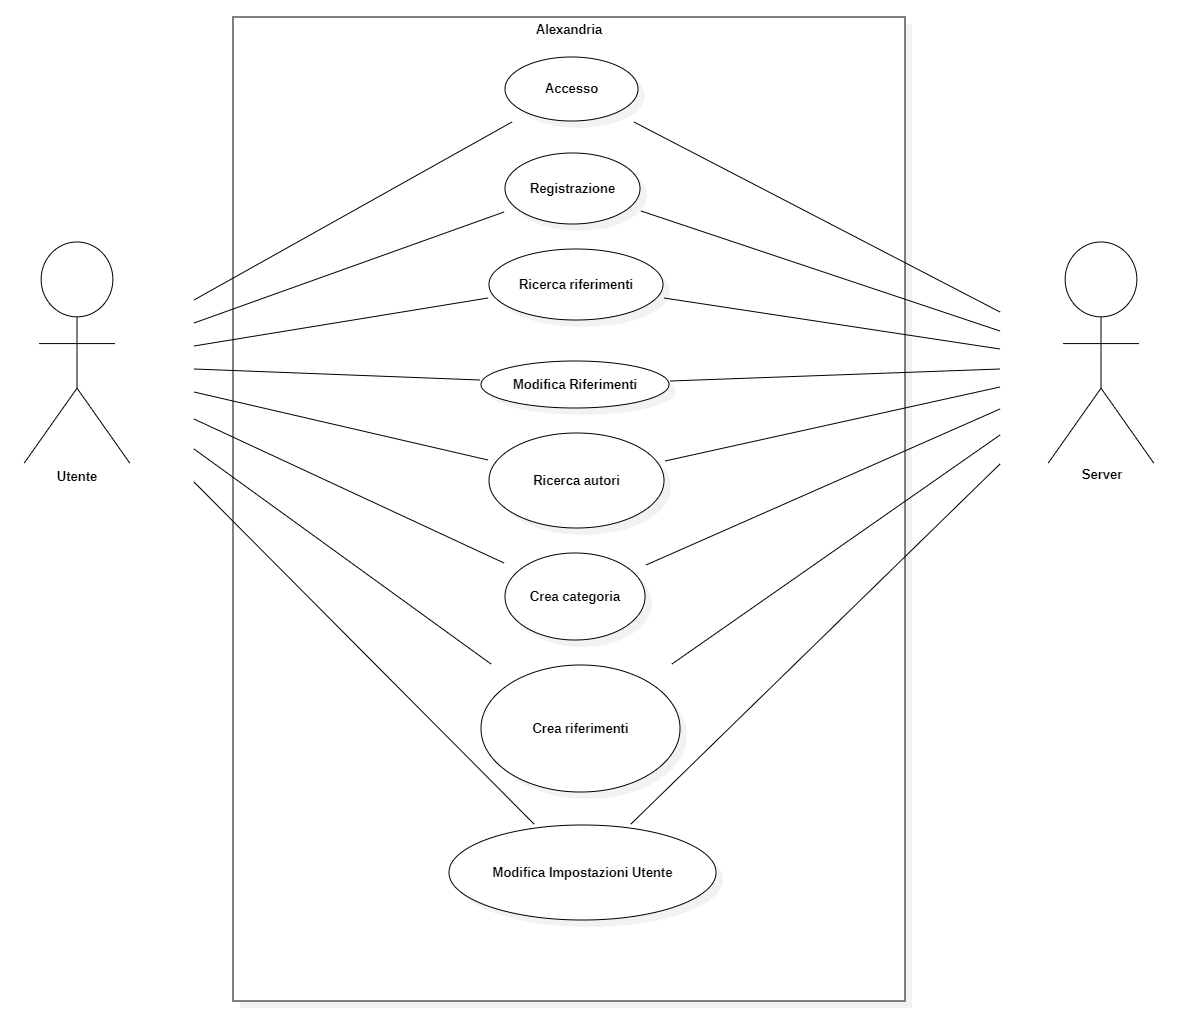
\includegraphics[width=.90\textwidth]{Immagini/Alexandria/useCase.png} 
        \end{center}
Il caso d'uso \textit{Accesso} permette l'autenticazione di un utente, ovvero permette ad un utente di accedere al sistema inserendo le proprie credenziali (scelte dall'utente stesso durante la fase di registrazione). Il caso d'uso \textit{Registrazione} permette di registrare un nuovo utente al sistema, scegliendo un proprio username, una propria password e una email. Il caso d'uso \textit{Ricerca Riferimenti} permette ad un utente di cercare un riferimento esistente nel sistema. Se inesistente, il sistema notifica l'utente dell'inesistenza del riferimento cercato, altrimenti permette di visualizzarlo. Il caso d'uso \textit{Modifica Riferimenti} permette ad un utente di modificare un riferimento creato in precedenza, in particolare permette di modificare un \gls{attributo} inserito in precedenza,  potendo scegliere un nuovo valore. Il caso d'uso \textit{Ricerca autori} permette all'utente di ricercare un autore in particolare e tutte le sue opere pubblicate presenti nel sistema. Il caso d'uso \textit{Crea categoria} permette all'utente di creare una categoria e di poter scegliere un'eventuale \gls{sopra-categoria}. Il caso d'uso \textit{Crea Riferimenti} permette ad un utente di creare un riferimento e di poterne assegnare gli attributi. Infine, il caso d'uso \textit{Modifica Impostazioni utente} permette ad un utente di modificare tutte le informazioni inserite durante la fase di registrazione.\\
Tutte queste funzionalità richiedono un attore esterno, ovvero il Server, il quale permette di registrare ogni modifica al sistema. Sostanzialmente, senza di esso l'applicativo non può funzionare correttamente.


\raggedright{\section{Individuazione target degli utenti}}
Il target principale degli utenti sono coloro i quali intendono gestire e visualizzare i propri riferimenti bibliografici. Per tale motivo Alexandria permette la gestione e la visualizzazione affidabile dei riferimenti creati. In aggiunta, è possibile visualizzare i riferimenti degli altri utenti presenti nel sistema.
Un altro possibile target di utenti sono gli autori stessi dei riferimenti bibliografici, poiché possono gestire facilmente le proprie opere pubblicate e visualizzarne gli attributi.
Un altro target di utenti sono le case editrici che intendono gestire le varie edizioni dei propri riferimenti pubblicati. 
Considerando tutti i possibili utenti, il team si impegna di poter soddisfare tutte le esigenze degli usufruitori e di poter garantire un'eccellente usabilità e affidabilità del sistema.

\raggedright{\section{4 casi d'uso in particolare}}
\raggedright{\subsection{Caso d'uso: Ricerca Riferimenti}}
\raggedright{\subsection{Caso d'uso: Creazione Riferimento}}
\raggedright{\subsection{Caso d'uso: Modifica propri Riferimenti}}
\raggedright{\subsection{Caso d'uso: Crea Categoria}}






\raggedright{\section{MockUp Interfaccia grafica}}

\raggedright{\section{Valutazione dell'usabilità}}

\raggedright{\section{Classi, oggetti e relazioni d'analisi}}

\raggedright{\section{Diagrammi di Sequenza}}

\raggedright{\section{Prototipazione funzionale}}









